\documentclass[11pt,a4paper]{report}

\usepackage[a4paper,
left=0.8in,
right=0.8in,
top=0.8in,
bottom=0.8in]{geometry}

\usepackage{graphicx}
\usepackage{amsmath}
\usepackage{amssymb}
\usepackage{booktabs}
\usepackage{array}
\usepackage{float}
\usepackage{tikz}
\usepackage{setspace}
\usepackage{hyperref}
\usepackage{titlesec}

\usepackage{listings}
\usepackage{xcolor}

\lstset{
language=C,
basicstyle=\ttfamily\scriptsize,
keywordstyle=\color{blue},
commentstyle=\color{green!50!black},
stringstyle=\color{red},
numbers=left,
numberstyle=\tiny,
frame=single,
breaklines=true,
showstringspaces=false
}

\usetikzlibrary{positioning,shapes.geometric,arrows.meta}

\setstretch{1.1}

\hypersetup{
colorlinks=true,
linkcolor=blue,
urlcolor=blue
}

\title{Report: Digital Clock Prototype}
\author{by Sanket Maniyar}
\date{}

\begin{document}

\maketitle

\tableofcontents

\newpage

\chapter{Digital Clock Prototype}

\section{Introduction}

The primary objective of this project was to design and implement a standalone digital clock using the ATmega328P microcontroller. The project integrated concepts of embedded systems, digital electronics and hardware interfacing into a functional real-time application. The clock displays time in the HH:MM format using a four-digit seven-segment display and allows the user to set the current time through dedicated push buttons.

The project also involved hardware debugging, software development, display multiplexing and enclosure design using Autodesk Fusion 360, thereby providing complete exposure to the embedded system development cycle.

%%%%%%%%%%%%%%%%%%%%%%%%%%%%%%%%%%%%%%%%%%%%%%%%%%%%%%%%%%

\section{Objectives}

The objectives of the project were:

\begin{itemize}
\item Design a standalone embedded system using the ATmega328P.
\item Interface a four-digit seven-segment display using GPIO pins.
\item Implement software-based timekeeping.
\item Allow manual time setting through push buttons.
\item Develop a compact enclosure using Autodesk Fusion 360.
\end{itemize}

%%%%%%%%%%%%%%%%%%%%%%%%%%%%%%%%%%%%%%%%%%%%%%%%%%%%%%%%%%

\section{System Architecture}

The digital clock consists of a standalone ATmega328P microcontroller, a four-digit seven-segment display, three push buttons, an external 16 MHz crystal oscillator and the supporting passive components. The microcontroller executes the timekeeping algorithm, scans the display using multiplexing and monitors user inputs.

\begin{figure}[H]
\centering

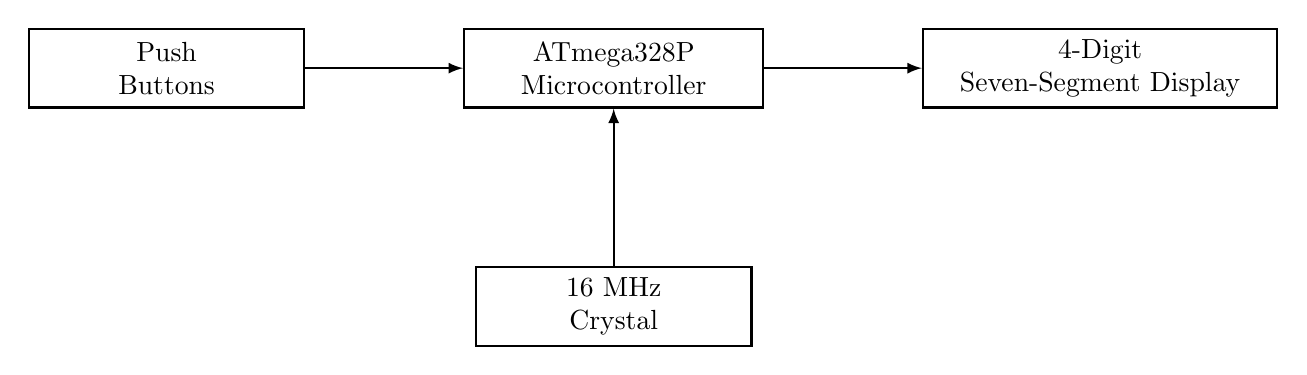
\begin{tikzpicture}[
node distance=2.2cm,
every node/.style={draw, thick, minimum height=1cm, align=center},
>=latex
]

\node (btn) [minimum width=3.5cm] {Push\\Buttons};

\node (mcu) [minimum width=3.8cm, right=2cm of btn] {ATmega328P\\Microcontroller};

\node (disp) [minimum width=4.5cm, right=2cm of mcu] {4-Digit\\Seven-Segment Display};

\node (xtal) [minimum width=3.5cm, below=2cm of mcu] {16 MHz\\Crystal};

\draw[->, thick] (btn) -- (mcu);
\draw[->, thick] (mcu) -- (disp);
\draw[->, thick] (xtal) -- (mcu);

\end{tikzpicture}

\caption{Block Diagram of the Digital Clock}
\end{figure}


%%%%%%%%%%%%%%%%%%%%%%%%%%%%%%%%%%%%%%%%%%%%%%%%%%%%%%%%%%

\section{Hardware Components}

\begin{table}[H]
\centering
\caption{Hardware Components Used}
\begin{tabular}{|l|c|}
\hline
Component & Quantity\\
\hline
ATmega328P Microcontroller & 1\\
Four-Digit Seven Segment Display & 1\\
16 MHz Crystal Oscillator & 1\\
Push Buttons & 3\\
330 $\Omega$ Resistors & 8\\
100 nF Capacitors & 2\\
220 pF Capacitors & 2\\
5 V Power Supply & 1\\
Breadboard/PCB & 1\\
\hline
\end{tabular}
\end{table}

%%%%%%%%%%%%%%%%%%%%%%%%%%%%%%%%%%%%%%%%%%%%%%%%%%%%%%%%%%

\section{Working Principle}

The ATmega328P maintains the current time through software counters driven by the external 16 MHz crystal oscillator. The four-digit seven-segment display is controlled using GPIO pins with multiplexing, where only one digit is activated at a time. Since the switching frequency is sufficiently high, persistence of vision makes all digits appear continuously illuminated.

Three push buttons provide user interaction.

\begin{itemize}
\item Hour Button – increments the hour.
\item Minute Button – increments the minute.
\item Start Button – starts normal clock operation after setting the time.
\end{itemize}

%%%%%%%%%%%%%%%%%%%%%%%%%%%%%%%%%%%%%%%%%%%%%%%%%%%%%%%%%%

\section{Software Flow}

\begin{figure}[H]
\centering

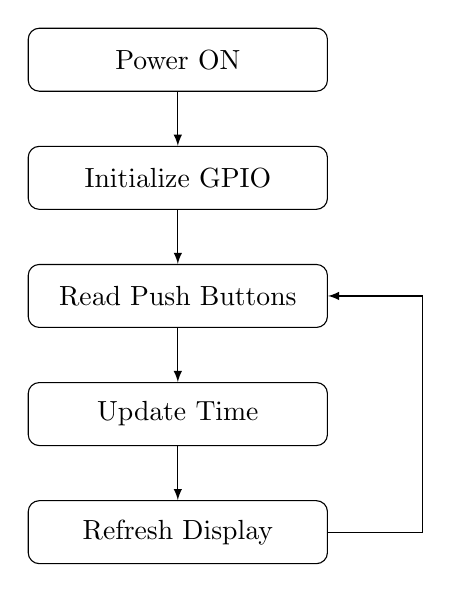
\begin{tikzpicture}[
node distance=1.5cm,
every node/.style={
draw,
rounded corners,
minimum width=3.8cm,
minimum height=0.8cm,
align=center
},
>=latex
]

\node (start) {Power ON};

\node (init) [below of=start] {Initialize GPIO};

\node (read) [below of=init] {Read Push Buttons};

\node (update) [below of=read] {Update Time};

\node (display) [below of=update] {Refresh Display};

\draw[->] (start) -- (init);
\draw[->] (init) -- (read);
\draw[->] (read) -- (update);
\draw[->] (update) -- (display);

% Loop back
\draw[->]
(display.east) -- ++(1.2,0)
|- (read.east);

\end{tikzpicture}

\caption{Software Flow of the Digital Clock}
\end{figure}

%%%%%%%%%%%%%%%%%%%%%%%%%%%%%%%%%%%%%%%%%%%%%%%%%%%%%%%%%%

\section{Implementation and Debugging}

The prototype was initially developed and tested using the Arduino development environment before programming the standalone ATmega328P microcontroller. GPIO pins were configured to control the display segments and read the push-button inputs.

Several practical challenges were encountered during implementation, including external crystal oscillator configuration, hardware wiring, stable display multiplexing and program uploading to the standalone microcontroller. These issues were resolved through systematic hardware verification and software debugging until reliable clock operation was achieved.

%%%%%%%%%%%%%%%%%%%%%%%%%%%%%%%%%%%%%%%%%%%%%%%%%%%%%%%%%%

\section{Firmware Development}

The firmware for the digital clock was developed in Embedded C using the Arduino IDE and programmed into the standalone ATmega328P microcontroller. The software initializes the GPIO pins, continuously refreshes the four-digit seven-segment display using multiplexing, reads the Hour, Minute and Start push buttons, and updates the displayed time every second.

Listing~\ref{lst:firmware} presents a representative portion of the firmware illustrating the initialization and main execution loop.

\begin{lstlisting}[caption={Main Firmware Structure},label={lst:firmware}]
const byte segPins[7]   = {2,3,4,5,6,7,8};
const byte digitPins[4] = {9,10,11,12};

const byte hourBtn   = A0;
const byte minuteBtn = A1;
const byte startBtn  = A2;

void setup()
{
    for(int i=0;i<7;i++)
        pinMode(segPins[i],OUTPUT);

    for(int i=0;i<4;i++)
        pinMode(digitPins[i],OUTPUT);

    pinMode(hourBtn,INPUT_PULLUP);
    pinMode(minuteBtn,INPUT_PULLUP);
    pinMode(startBtn,INPUT_PULLUP);
}

void loop()
{
    readButtons();
    updateClock();
    refreshDisplay();
}
\end{lstlisting}

The complete firmware consists of multiple functions responsible for GPIO initialization, button handling, software-based timekeeping and display multiplexing. Only the main program structure is included here for brevity.

\section{Prototype}

\begin{figure}[H]
\centering
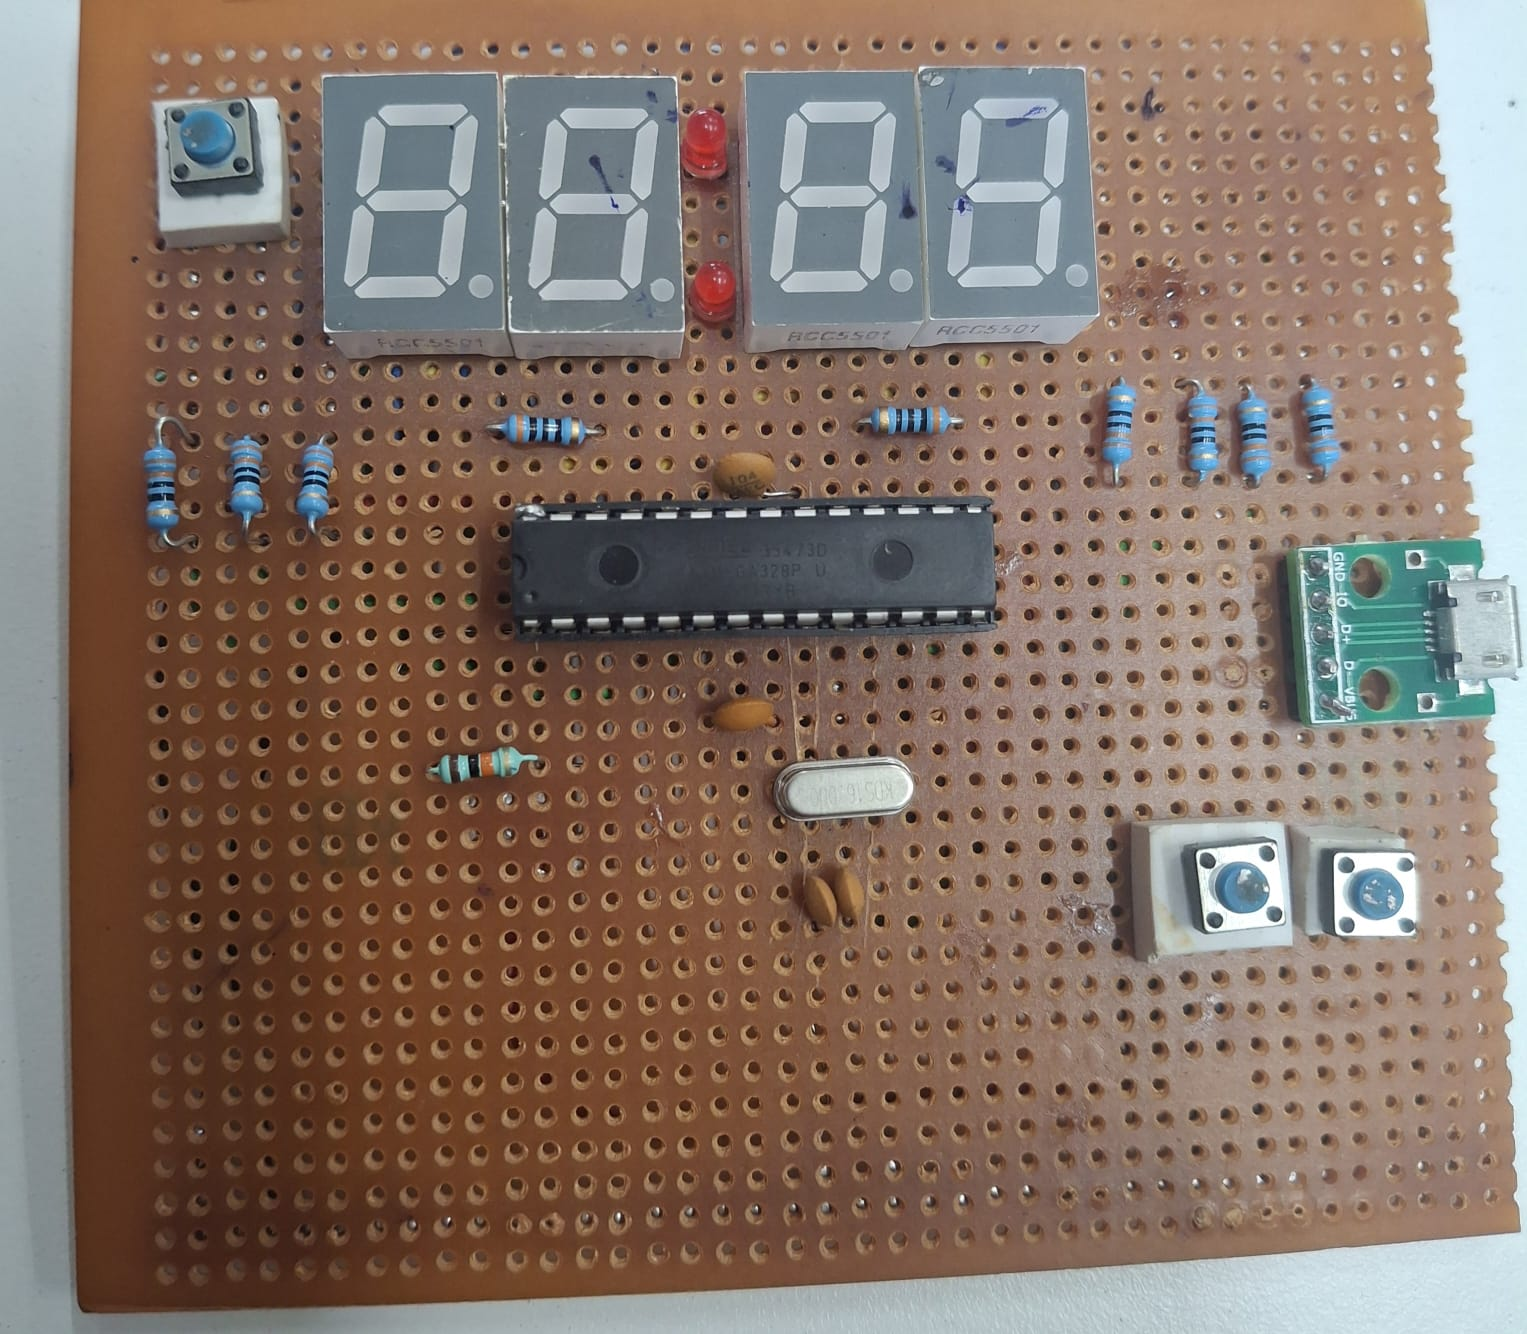
\includegraphics[width=0.8\textwidth]{clock.jpeg}
\caption{Completed Digital Clock Prototype}
\end{figure}

%%%%%%%%%%%%%%%%%%%%%%%%%%%%%%%%%%%%%%%%%%%%%%%%%%%%%%%%%%

\section{Fusion 360 Enclosure Design}

To improve the appearance and protection of the prototype, a custom enclosure was designed using Autodesk Fusion 360. The enclosure was modeled to accommodate the display, push buttons and power connections while providing adequate structural support for the electronic components. The CAD model can be directly used for fabrication using additive manufacturing techniques such as 3D printing.

\begin{figure}[H]
\centering
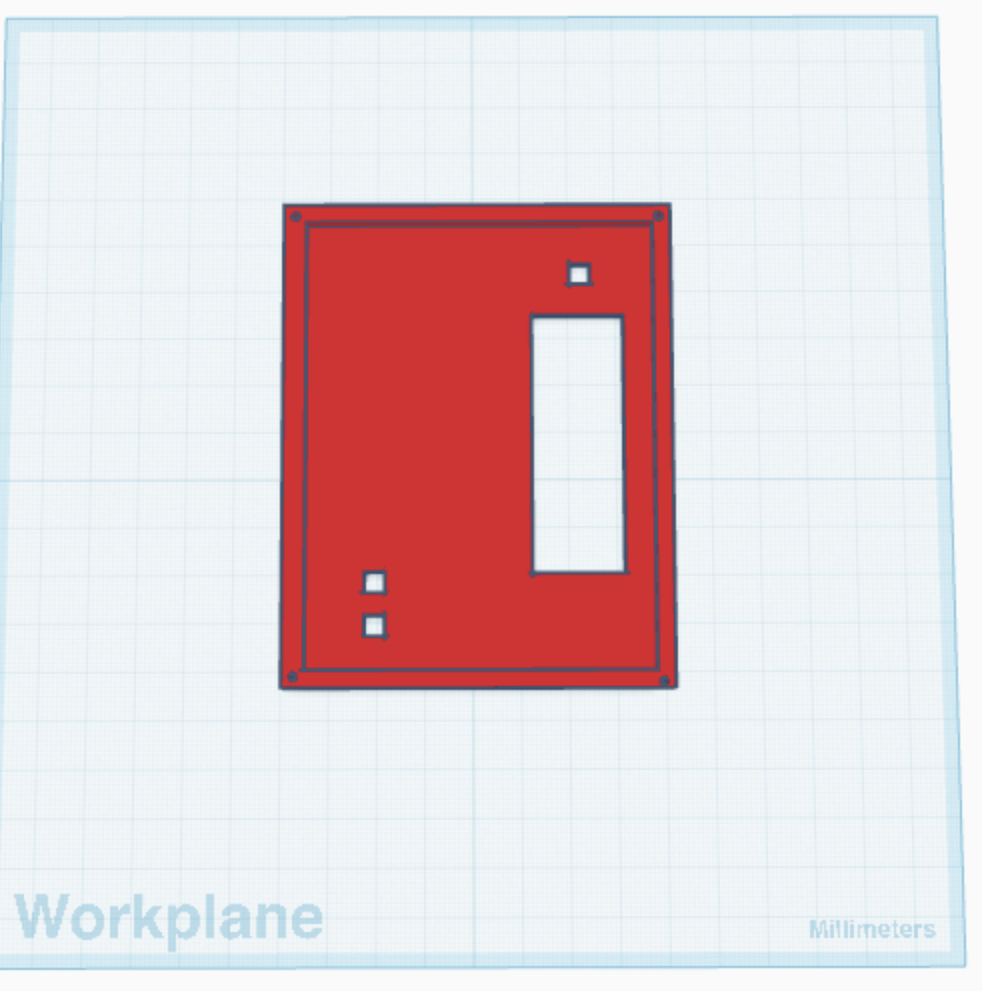
\includegraphics[width=0.8\textwidth]{top.png}
\caption{Fusion 360 Model of the Enclosure-Top}
\end{figure}

\begin{figure}[H]
\centering
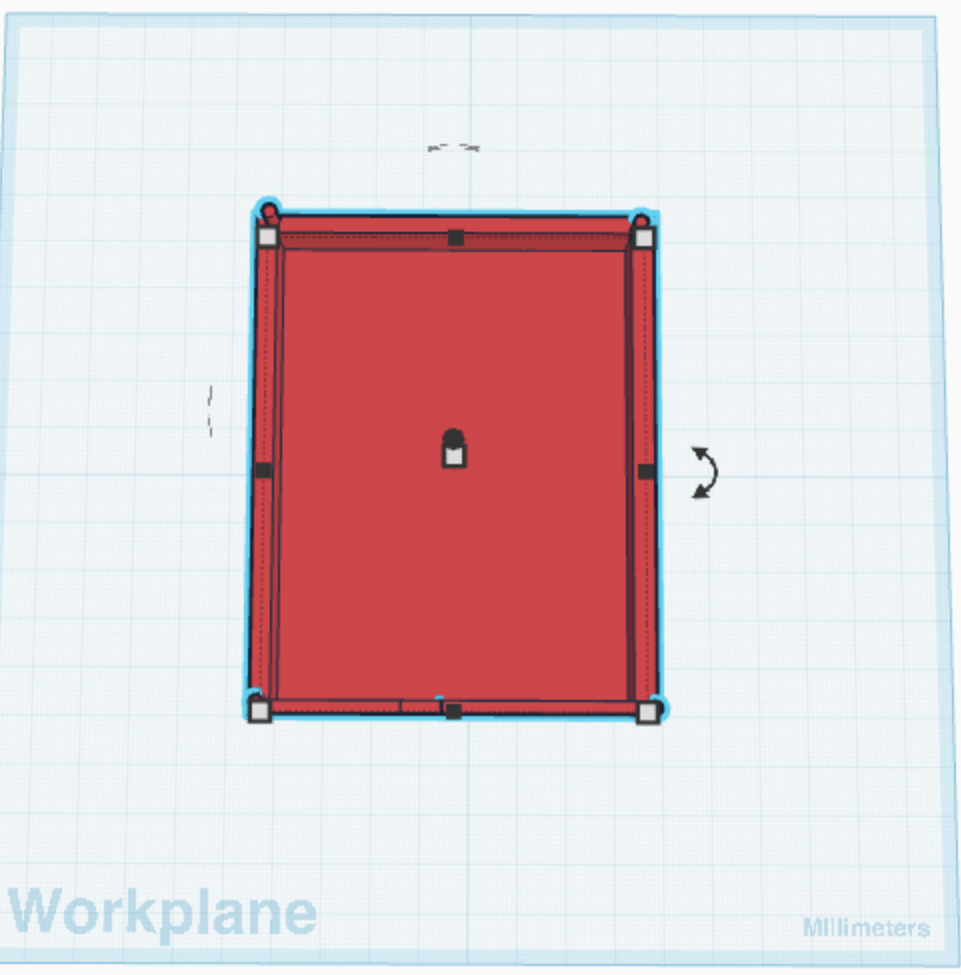
\includegraphics[width=0.8\textwidth]{bottom.png}
\caption{Bottom}
\end{figure}

%%%%%%%%%%%%%%%%%%%%%%%%%%%%%%%%%%%%%%%%%%%%%%%%%%%%%%%%%%

\section{Results}

The digital clock successfully displayed time in the HH:MM format using a standalone ATmega328P microcontroller. The Hour, Minute and Start buttons functioned as intended, allowing the user to configure and operate the clock. The multiplexed display produced stable, flicker-free output, while the external crystal oscillator ensured reliable timekeeping. The enclosure designed using Fusion 360 complemented the hardware by providing a compact and organized mechanical structure.

%%%%%%%%%%%%%%%%%%%%%%%%%%%%%%%%%%%%%%%%%%%%%%%%%%%%%%%%%%

\section{Conclusion}

The digital clock project successfully integrated embedded programming, digital electronics and mechanical design into a complete embedded system. The project strengthened practical understanding of GPIO interfacing, display multiplexing, hardware debugging and standalone microcontroller implementation. In addition to achieving the intended functionality, the project demonstrated the complete workflow involved in designing, implementing and packaging an embedded hardware prototype.

\end{document}